\section{Expert Reviews / Inspections}

Per valutare la qualità complessiva dell’esperienza utente e la coerenza progettuale del sistema, è stata pianificata una revisione sistematica dell’interfaccia basata su una \textbf{valutazione euristica} secondo i principi di Nielsen \cite{nielsen1995}.  
L’attività ha avuto l’obiettivo di identificare punti di forza, criticità e incoerenze nel design, analizzando in due fasi distinte il \textit{prototipo realizzato in Figma} e successivamente la \textit{versione web implementata}.  

La revisione del prototipo Figma ha rappresentato un passaggio fondamentale prima dello sviluppo effettivo: ha consentito di riflettere in modo critico sulle scelte di interfaccia, di validare le principali logiche di navigazione e di anticipare eventuali problemi di usabilità.  
A differenza della versione web, il prototipo non consente un’interazione reale, ma offre comunque una base solida per verificare la chiarezza dei flussi e la coerenza visiva complessiva.

\subsection*{Obiettivi della Review}

Gli obiettivi principali dell’attività di \textit{Expert Review} sono stati:
\begin{itemize}
    \item Valutare la \textbf{usabilità} dei flussi principali del sistema, verificando la chiarezza dei percorsi e delle azioni disponibili.
    \item Analizzare la \textbf{coerenza visiva} rispetto alle linee guida di design definite nel brand e nel prototipo.
    \item Individuare problemi di \textbf{chiarezza, navigabilità e feedback} che possano compromettere l’esperienza d’uso.
    \item Identificare eventuali mancanze o ridondanze, con l’obiettivo di \textbf{migliorare la struttura informativa e la consistenza visiva}.
    \item Definire raccomandazioni per le fasi successive di sviluppo, in vista della revisione della \textbf{versione web funzionante}.
\end{itemize}

\subsection*{Motivazione della Checklist Scelta}

Per garantire una valutazione sistematica, replicabile e comparabile tra diverse aree dell’interfaccia, è stata utilizzata una \textbf{checklist di usabilità} costruita sui dieci principi di Nielsen.  
Questo approccio è stato scelto perché:
\begin{itemize}
    \item consente una \textbf{autovalutazione strutturata} anche in assenza di utenti reali o revisori esterni;
    \item può essere applicato sia a \textbf{prototipi statici} (come quelli sviluppati in Figma) sia a \textbf{interfacce interattive} e funzionanti;
    \item copre in modo ampio le dimensioni fondamentali dell’usabilità: visibilità dello stato del sistema, coerenza, prevenzione degli errori, efficienza, chiarezza e supporto all’utente.
\end{itemize}

\subsection*{Struttura della Checklist Euristica}

La checklist adottata si basa sui dieci principi classici di Nielsen, riformulati in forma di domande operative per adattarli al contesto del progetto.  
Ogni criterio è stato utilizzato come base per analizzare il prototipo Figma e successivamente la versione web.

\begin{table}[H]
\centering
\begin{tabular}{p{0.7cm} p{4cm} p{8cm}}
\hline
\textbf{\#} & \textbf{Criterio} & \textbf{Domanda di verifica} \\
\hline
1 & Visibilità dello stato del sistema & L’utente riceve sempre un feedback visivo o testuale dopo un’azione (salvataggio, invio, errore)? \\
2 & Corrispondenza tra sistema e mondo reale & Terminologia, icone e messaggi sono coerenti con il linguaggio del dominio immobiliare? \\
3 & Controllo e libertà dell’utente & È possibile annullare o correggere facilmente un’azione? \\
4 & Coerenza e standard & Colori, stili e componenti rispettano il design definito nel brand e nel prototipo? \\
5 & Prevenzione e gestione degli errori & I form prevengono gli errori tramite validazioni e messaggi chiari? \\
6 & Efficienza e flessibilità d’uso & Le operazioni più frequenti possono essere eseguite rapidamente, anche da dispositivi mobili? \\
7 & Chiarezza del contenuto & Testi e etichette sono comprensibili e privi di ambiguità? \\
8 & Supporto al riconoscimento & Le opzioni principali sono visibili e non richiedono memoria a breve termine all’utente? \\
9 & Feedback e conferme & Sono presenti messaggi di conferma dopo azioni critiche (pubblicazione, eliminazione, invio)? \\
10 & Aiuto e documentazione & È disponibile un supporto o una guida per l’utente in caso di difficoltà? \\
\hline
\end{tabular}
\caption{Checklist di valutazione euristica basata sui principi di Nielsen.}
\end{table}

\bigskip

La sezione seguente presenta nel dettaglio l’applicazione di questa checklist al \textbf{prototipo Figma}, con un’analisi critica dei dieci criteri e una successiva autovalutazione sintetica dei risultati ottenuti.

\subsection{Expert Review sul Prototipo Figma}

L’attività di revisione euristica è stata condotta sul prototipo sviluppato in \textit{Figma} prima della realizzazione della versione web.  
L’obiettivo è stato valutare il livello di usabilità e coerenza delle principali interfacce progettate, verificando la presenza di feedback, la chiarezza dei flussi e la consistenza grafica secondo i dieci principi di Nielsen.  

\subsubsection*{1. Visibilità dello stato del sistema}  
Nel prototipo sono stati previsti diversi meccanismi di feedback.  
Nei flussi \textit{Fai controproposta} e \textit{Registra dipendente} sono stati inseriti \textbf{indicatori di caricamento} per mostrare lo stato del sistema durante le operazioni.  
In tutti i form è presente un \textbf{sistema di validazione immediata}: i campi non validi vengono evidenziati in rosso e, nel caso della \textit{creazione di un annuncio}, il processo è suddiviso in step.  
Quando uno step contiene errori, il suo indicatore cambia colore e un box iniziale riepiloga i campi non validi.  
Tutti i flussi analizzati includono un \textbf{doppio messaggio di conferma} prima dell’esecuzione definitiva, ad eccezione della creazione di un annuncio.  
Nel complesso, il prototipo offre una buona visibilità dello stato del sistema, con l’unica criticità relativa all’assenza di conferma dopo la pubblicazione.

\subsubsection*{2. Corrispondenza tra sistema e mondo reale}  
Il linguaggio utilizzato è \textbf{semplice e diretto}, adatto agli utenti finali.  
Le sezioni con terminologia più specifica (legate alle agenzie immobiliari) risultano coerenti con il dominio e adatte a un pubblico professionale.  
Sono state impiegate \textbf{icone standard e universalmente riconoscibili}, affiancate da \textbf{tooltip descrittivi} che ne chiariscono il significato.  
L’unico aspetto ancora da migliorare riguarda la \textbf{scelta delle icone nello stepper} di creazione annuncio, dove sarebbe utile uno studio mirato per rendere più intuitivi i passaggi.

\subsubsection*{3. Controllo e libertà dell’utente}  
Il prototipo garantisce buone possibilità di annullamento e controllo.  
Tutti i popup includono una \textbf{“X” per chiudere o annullare}, e i messaggi di conferma prevedono esplicitamente un pulsante \textit{Annulla}.  
Le azioni potenzialmente distruttive, come la \textbf{disattivazione delle notifiche}, richiedono conferma; viceversa, l’attivazione non la richiede poiché non comporta rischi di perdita di dati.  
La progettazione su questo punto è stata ritenuta soddisfacente e coerente con le aspettative di usabilità.

\subsubsection*{4. Coerenza e standard}  
Il design mantiene nel complesso una \textbf{coerenza visiva} nei colori e nello stile dei pulsanti, in linea con il concept minimalista del progetto.  
Tuttavia, si è rilevata una \textbf{mancanza di uniformità nei popup}: nei diversi casi d’uso sono stati utilizzati modelli leggermente differenti, frutto di sperimentazioni grafiche ancora non consolidate.  
In fase di sviluppo sarà necessario \textbf{uniformare componenti e modali}, garantendo una coerenza piena tra tutti i flussi.

\subsubsection*{5. Prevenzione e gestione degli errori}  
La prevenzione degli errori è uno degli aspetti più curati nel prototipo.  
I form mostrano in tempo reale i campi non validi e forniscono \textbf{indicazioni visive chiare (rosso)} insieme a messaggi testuali.  
La combinazione di validazione immediata e conferme d’azione riduce significativamente il rischio di errori da parte dell’utente.  
Questo punto risulta pienamente soddisfatto.

\subsubsection*{6. Efficienza e flessibilità d’uso}  
Essendo un prototipo statico, l’efficienza d’uso è valutabile solo in parte.  
L’interfaccia è stata progettata per un utilizzo anche da \textbf{dispositivi verticali}, ma la resa migliore si ottiene in \textbf{orientamento orizzontale (landscape)}.  
Non sono state ancora considerate \textbf{scorciatoie o funzionalità avanzate} per utenti esperti (es. salvataggio bozza, importazione di dati da file), che potrebbero rappresentare un’evoluzione futura del progetto.  
Si riconosce quindi questo come un punto da sviluppare ulteriormente.

\subsubsection*{7. Chiarezza del contenuto}  
I testi sono \textbf{brevi, diretti e privi di tecnicismi}, con un linguaggio coerente e immediato.  
Quando una sola etichetta non è sufficiente, è previsto l’uso di \textbf{tooltip esplicativi}.  
Questo approccio consente una buona comprensione del flusso anche senza documentazione aggiuntiva.

\subsubsection*{8. Supporto al riconoscimento}  
Le principali funzioni sono \textbf{raggiungibili in pochi clic}.  
La \textit{header bar} consente di passare rapidamente tra ricerca, storico annunci e notifiche; inoltre, il passaggio tra l’area cliente e quella agenzia è reso accessibile dal \textit{footer}.  
Un test di eye-tracking condotto su alcune schermate del prototipo ha confermato la \textbf{corretta collocazione visiva} degli elementi più rilevanti, validando l’efficacia della struttura.

\subsubsection*{9. Feedback e conferme}  
Le operazioni critiche, come eliminazione o modifica, utilizzano lo stesso colore principale del sito, il che può generare confusione con azioni neutre.  
Si suggerisce di differenziare \textbf{visivamente le azioni distruttive} (es. usando toni di rosso o arancione) e di inserire messaggi di conferma più evidenti per i processi più delicati.  
Nonostante ciò, il comportamento rimane accettabile per utenti esperti.

\subsubsection*{10. Aiuto e documentazione}  
Non è stato previsto un sistema di aiuto, documentazione o FAQ, poiché il prototipo nasce in un contesto accademico.  
Tuttavia, in una versione completa sarebbe opportuno introdurre:  
\begin{itemize}
    \item una \textbf{sezione FAQ} o assistenza per i problemi più comuni;  
    \item \textbf{overlay o onboarding guidato} per i nuovi utenti;  
    \item pulsanti contestuali “Come funziona” nelle pagine più complesse.  
\end{itemize}

\subsubsection*{Autovalutazione e sintesi}  
La tabella seguente riassume il livello di soddisfacimento delle euristiche sul prototipo Figma (0 = non soddisfatto, 1 = parzialmente soddisfatto, 2 = soddisfatto).

\begin{table}[h!]
\centering
\begin{tabular}{p{0.4cm} p{4cm} p{1.5cm} p{7cm}}
\hline
\textbf{\#} & \textbf{Criterio} & \textbf{Valutazione} & \textbf{Motivazione sintetica} \\ \hline
1 & Visibilità stato & 2 & Feedback e validazioni chiare, manca solo conferma finale in creazione annuncio \\
2 & Corrispondenza mondo reale & 2 & Linguaggio semplice e coerente, icone chiare \\
3 & Controllo e libertà & 2 & Annulla e conferme sempre presenti \\
4 & Coerenza e standard & 1 & Popup non uniformi tra i flussi \\
5 & Prevenzione errori & 2 & Validazione in tempo reale e segnalazioni visive \\
6 & Efficienza/flessibilità & 1 & Assenza di scorciatoie e ottimizzazione solo parziale per mobile \\
7 & Chiarezza del contenuto & 2 & Testi sintetici e coerenti \\
8 & Supporto al riconoscimento & 2 & Navigazione semplice e confermata da test visivi \\
9 & Feedback/Conferme & 1 & Colori azioni critiche da differenziare \\
10 & Aiuto/Documentazione & 0 & Non prevista sezione di supporto \\ \hline
\end{tabular}
\caption{Autovalutazione euristica del prototipo Figma secondo i principi di Nielsen.}
\end{table}

\subsubsection*{Conclusioni}  
Il prototipo Figma risulta \textbf{completo, coerente e ben strutturato}, con una gestione accurata dei form, validazioni efficaci e buona leggibilità generale.  
I principali margini di miglioramento riguardano la \textbf{coerenza visiva dei popup}, la \textbf{differenziazione dei feedback critici} e l’assenza di un \textbf{sistema di aiuto} o onboarding.  
Questi aspetti costituiranno la base per le iterazioni successive e per l’ottimizzazione della versione web finale.



TODO Da fare bene la seocnda parte 

\textbf{Versione Web:} la checklist è stata applicata all’intero insieme di requisiti e funzionalità richiesti dal docente, permettendo una valutazione completa dell’interfaccia e dei flussi principali del sistema.

\subsection*{Definizione della Checklist di Usabilità}

La checklist elaborata si basa su una selezione adattata delle euristiche di Nielsen, ridotte e riformulate per meglio aderire al contesto del progetto.  
Ogni criterio è espresso come domanda di verifica utilizzata per valutare sia il prototipo sia il sito web.

\begin{table}[h!]
\centering
\begin{tabular}{p{0.8cm} p{4cm} p{7cm}}
\hline
\textbf{\#} & \textbf{Criterio} & \textbf{Domanda di verifica} \\
\hline
1 & Visibilità dello stato del sistema & L’utente riceve sempre un feedback visivo o testuale in seguito a un’azione (es. salvataggio, invio, errore)? \\
2 & Corrispondenza tra sistema e mondo reale & Terminologia, icone e messaggi sono coerenti con il linguaggio del dominio immobiliare? \\
3 & Controllo e libertà dell’utente & È possibile annullare o correggere facilmente un’azione (es. modifica o cancellazione di un annuncio)? \\
4 & Coerenza e standard & Colori, stili e pulsanti rispettano il design definito nel brand e nel prototipo Figma? \\
5 & Prevenzione e gestione degli errori & I form prevengono errori tramite validazioni e messaggi chiari? \\
6 & Efficienza e flessibilità d’uso & Le operazioni più frequenti possono essere completate rapidamente e da dispositivi mobili verticali? \\
7 & Chiarezza del contenuto & I testi e le etichette guidano l’utente nel flusso, senza ambiguità? \\
8 & Supporto al riconoscimento & Le opzioni principali sono sempre visibili senza richiedere memoria a breve termine all’utente? \\
9 & Feedback e conferme & Sono presenti messaggi di conferma dopo operazioni critiche (es. pubblicazione, eliminazione, invio)? \\
10 & Aiuto e documentazione & È disponibile una sezione informativa o un supporto base per l’utente? \\
\hline
\end{tabular}
\caption{Checklist di usabilità basata sulle euristiche di Nielsen, adattata al contesto del sito immobiliare multi-agenzia.}
\label{tab:checklist_usabilita}
\end{table}

\subsection*{Applicazione della Checklist}

La review è stata eseguita individualmente per ciascun caso d’uso su Figma e per l’intero insieme di funzionalità sulla versione web.  
I risultati sono stati successivamente confrontati per identificare le criticità più significative e le aree di miglioramento.




Questo capitolo è suddiviso in due sezioni principali. Nella prima sezione vengono illustrate le strategie adottate per l’esecuzione dei test unitari utilizzando il framework xUnit, con particolare attenzione alla definizione delle classi di equivalenza, alla copertura dei percorsi logici e all’individuazione dei casi limite. Nella seconda sezione vengono presentate le valutazioni sull’usabilità del sistema, con analisi dei test condotti sugli utenti finali e delle metodologie adottate per misurare l’efficacia, l’efficienza e la soddisfazione nell’utilizzo dell’applicazione.

\section{Progettazione e implementazione dei test unitari}

Per la fase di unit testing sono stati selezionati i seguenti metodi da sottoporre a verifica:

\begin{itemize}
	\item NewDipendenteResponse addDipendente(DipendenteRequest request, String aliasAgenzia)
	\item List<ContattoResponse> aggiungiContatto(ContattoRequest request)
	\item String changePassword(String oldPassword, String newPassword, String confirmPassword)
	\item List<User> utentiInteressati(CriteriDiRicercaUtenti request)
\end{itemize}

\section{addDipendente(DipendenteRequest request, String aliasAgenzia)}

Il metodo \textit{addDipendente}, appartenente alla classe UserService, ha la responsabilità di aggiungere al sistema un nuovo dipendente, che può essere un agente o un manager.

Per questo metodo è stata adottata una strategia di\textbf{ Black Box} Testing, poiché l’obiettivo principale è verificare il comportamento del sistema in base agli stati e ai valori dei parametri in ingresso, senza considerare la logica interna dell’implementazione. In particolare, si è ritenuto fondamentale analizzare le diverse condizioni in cui un dipendente viene correttamente registrato o rifiutato dal sistema.

A tal fine, è stata effettuata una suddivisione dei parametri di input in \textbf{classi di equivalenza}, al fine di individuare i casi validi e non validi da sottoporre a test. Di seguito si riportano le tabelle che documentano tale suddivisione:

\begin{table}[H]
	\centering
	\begin{tabular}{|c|p{4cm}|p{5cm}|c|} 
		\hline
		\textbf{ID Classe} & \textbf{Descrizione} & \textbf{Valore esempio} & \textbf{Validità} \\
		\hline
		DRN1 & L'insieme delle stringe non vuote/lunghezza zero
		& request.nome==Roberto; & Valido \\
		\hline
		DRN2 & L'insieme delle stringhe null/lunghezza zero
		& request.nome=="" & Non Valido \\
		\hline
	\end{tabular}
	\caption{Parametro DipendenteRequest.nome}
	\label{tab:parametriDipendenteRequestNome}
\end{table}

\begin{table}[H]
	\centering
	\begin{tabular}{|c|p{6cm}|p{5cm}|c|} 
		\hline
		\textbf{ID Classe} & \textbf{Descrizione} & \textbf{Valore esempio} & \textbf{Validità} \\
		\hline
		DRC1 & L'insieme delle stringe non vuote/lunghezza zero
		& request.cognome==Morosini; & Valido \\
		\hline
		DRC2 & L'insieme delle stringhe null/lunghezza zero
		& request.cognome==null & Non Valido \\
		\hline
	\end{tabular}
	\caption{Parametro DipendenteRequest.cognome}
	\label{tab:parametriDipendenteRequestCognome}
\end{table}

\begin{table}[H]
	\centering
	\begin{tabular}{|c|p{4cm}|p{5.5cm}|c|} 
		\hline
		\textbf{ID Classe} & \textbf{Descrizione} & \textbf{Valore esempio} & \textbf{Validità} \\
		\hline
		DRR1 & Stringa di valore "AGENT"
		& request.ruolo=="AGENT"; & Valido \\
		\hline
		DRR2 & Stringa di valore "MANAGER"
		& request.ruolo=="MANAGER" & Valido \\
		\hline
		DRR3 & tutti i valori non corrispodenti ad AGENT oppure a MANAGER
		& request.ruolo=="ADMIN" & Non Valido \\
		\hline
		DRR4 & stringa null/lunghezza zero
		& request.ruolo=="" & Non Valido \\
		\hline
	\end{tabular}
	\caption{Parametro DipendenteRequest.ruolo}
	\label{tab:parametriDipendenteRequestRuolo}
\end{table}

\begin{table}[H]
	\centering
	\begin{tabular}{|c|p{4cm}|p{5.5cm}|c|} 
		\hline
		\textbf{ID Classe} & \textbf{Descrizione} & \textbf{Valore esempio} & \textbf{Validità} \\
		\hline
		AA1 & L'insieme delle stringhe non null e non vuoti & aliasAgenzia==RobyImmobili & Valida \\
		\hline
		AA2 & La stringa è null oppure è vuota & aliasAgenzia==null & Non valido \\
		\hline
	\end{tabular}
	\caption{Parametro aliasAgenzia}
	\label{tab:parametriAliasAgenzia}
\end{table}

\vspace{1cm}

Per quanto riguarda la strategia di combinazione dei valori, è stato scelto l’approccio \textbf{R-WECT (Reduced Weak Equivalence Class Testing)}. Questa tecnica è considerata particolarmente robusta perché garantisce:

\begin{itemize}
	\item il test di tutte le classi non valide, ognuna combinata con valori validi per gli altri parametri;
	\item il test di tutte le classi valide per ciascun parametro.
\end{itemize}

Infine, vengono riportati sia il codice sorgente dei test implementati sia l’evidenza del loro esito positivo, a conferma della correttezza delle funzionalità verificate

% Definizione dei colori
\definecolor{bgcolor}{RGB}{245,245,245}    % Sfondo chiaro
\definecolor{keywordcolor}{RGB}{0,0,180}  % Blu per le parole chiave
\definecolor{commentcolor}{RGB}{0,128,0}  % Verde per i commenti
\definecolor{stringcolor}{RGB}{163,21,21} % Rosso per le stringhe

% Configurazione listings
\lstset{
	language=Java,                % Linguaggio di esempio
	backgroundcolor=\color{bgcolor}, % Colore di sfondo
	basicstyle=\ttfamily\small,     % Font e dimensione
	keywordstyle=\color{keywordcolor}\bfseries,
	commentstyle=\color{commentcolor}\itshape,
	stringstyle=\color{stringcolor},
	numbers=left,                   % Numeri a sinistra
	numberstyle=\tiny\color{gray},  % Stile dei numeri
	stepnumber=1,                   % Numeri in ogni riga
	numbersep=5pt,                  % Distanza dai numeri
	frame=single,                   % Cornice intorno al codice
	rulecolor=\color{gray},         % Colore della cornice
	tabsize=4,                       % Tab = 4 spazi
	showstringspaces=false,
	breaklines=true,                  % A capo automatico se troppo lungo
	literate=
		{à}{{\`a}}1
		{è}{{\`e}}1
		{é}{{\'e}}1
		{ì}{{\`i}}1
		{ò}{{\`o}}1
		{ù}{{\`u}}1
}


\begin{lstlisting}
/**
* Test che copre le classi valide: DRN1 (Valida); DRC1 (Valida); DRR1(Valida); AA1(Valida);
*/
@Test
void addDipedenteTestAddAgente(){
	
	DipendenteRequest dipendente = new DipendenteRequest("Roberto", "Spena", "AGENT");
	String dominioAgenzia = "RobyImmobili";
	
	when(userRepository.countByEmail("roberto.spena@robyimmobili.dietiestate.com")).thenReturn(0);
	
	Authority fakeAuthority = new Authority();
	fakeAuthority.setAuthorityName(AuthorityName.AGENT);
	when(authorityRepository.findByAuthorityName(AuthorityName.AGENT)).thenReturn(Optional.of(fakeAuthority));
	
	User fakeUser = new User();
	fakeUser.setId(1); //id fittizio
	DatiImpiegato fakeDati = new DatiImpiegato();
	when(userRepository.save(Mockito.any(User.class))).thenReturn(fakeUser);
	when(datiImpiegatoRepository.save(Mockito.any(DatiImpiegato.class))).thenReturn(fakeDati);
	
	NewDipendeteResponse response = userService.addDipendete(dipendente,dominioAgenzia);
	
	//Controllo email generata
	String emailPrevista = "roberto.spena@robyimmobili.dietiestate.com";
	assertEquals(emailPrevista, response.getUser().getEmail(), "Email non generata correttamente");
	
	//Controllo password generata
	String password = response.getPassword();
	assertEquals(12, password.length(), "La password deve essere lunga 12 caratteri");
	assertTrue(
	password.matches(".*[a-zA-Z].*"),
	"La stringa deve contenere almeno una lettera"
	);
	assertTrue(
	password.matches(".*[!@#$%^&*()\\\\-_=+\\\\[\\\\]{}|;:,.<>?].*"),
	"La stringa deve contenere almeno un carattere speciale"
	);
	assertTrue(
	password.matches(".*[0-9].*"),
	"La stringa deve contenere almeno una cifra"
	);
	
	//Controllo nomeVisualizzato
	String nomeVisualizzato = response.getUser().getNomeVisualizzato();
	String nomeVisualizzatoPrevisto = "Agente Roberto S.";
	assertEquals(nomeVisualizzato, nomeVisualizzatoPrevisto);
	
	//Controllo foto profilo
	String fotoProfilo = response.getUser().getUrlFotoProfilo();
	assertTrue(fotoProfilo.matches("^https://dummyimage.com/.*"), "Url foto profilo non valido");
}
\end{lstlisting}

\begin{lstlisting}
	/**
	*  Test che copre le classi valide: DRN1 (Valida); DRC1 (Valida); DRR2(Valida); AA1(Valida);
	*/
	@Test
	void addDipedenteTestAddManager(){
		
		DipendenteRequest dipendente = new DipendenteRequest("Raimondo", "Morosini", "MANAGER");
		String dominioAgenzia = "RaimondoImmobili";
		
		when(userRepository.countByEmail("raimondo.morosini@raimondoimmobili.dietiestate.com")).thenReturn(0);
		
		Authority fakeAuthority = new Authority();
		fakeAuthority.setAuthorityName(AuthorityName.MANAGER);
		when(authorityRepository.findByAuthorityName(AuthorityName.MANAGER)).thenReturn(Optional.of(fakeAuthority));
		
		User fakeUser = new User();
		fakeUser.setId(1); //id fittizio
		DatiImpiegato fakeDati = new DatiImpiegato();
		when(userRepository.save(Mockito.any(User.class))).thenReturn(fakeUser);
		when(datiImpiegatoRepository.save(Mockito.any(DatiImpiegato.class))).thenReturn(fakeDati);
		
		NewDipendeteResponse response = userService.addDipendete(dipendente,dominioAgenzia);
		
		//Controllo email generata
		String emailPrevista = "raimondo.morosini@raimondoimmobili.dietiestate.com";
		assertEquals(emailPrevista, response.getUser().getEmail(), "Email non generata correttamente");
		
		//Controllo password generata
		String password = response.getPassword();
		assertEquals(12, password.length(), "La password deve essere lunga 12 caratteri");
		assertTrue(
		password.matches(".*[a-zA-Z].*"),
		"La stringa deve contenere almeno una lettera"
		);
		assertTrue(
		password.matches(".*[!@#$%^&*()\\\\-_=+\\\\[\\\\]{}|;:,.<>?].*"),
		"La stringa deve contenere almeno un carattere speciale"
		);
		assertTrue(
		password.matches(".*[0-9].*"),
		"La stringa deve contenere almeno una cifra"
		);
		
		//Controllo nomeVisualizzato
		String nomeVisualizzato = response.getUser().getNomeVisualizzato();
		String nomeVisualizzatoPrevisto = "Manager Raimondo M.";
		assertEquals(nomeVisualizzato, nomeVisualizzatoPrevisto);
		
		//Controllo foto profilo
		String fotoProfilo = response.getUser().getUrlFotoProfilo();
		assertTrue(fotoProfilo.matches("^https://dummyimage.com/.*"), "Url foto profilo non valido");
	}
\end{lstlisting}

\begin{lstlisting}
	/**
	* Test per coprire la classe nome non valida: DRN1 (Non Valida); DRC1 (Valida); DRR2(Valida); AA1(Valida);
	*/
	@Test
	void addDipedenteTestNomeNonValido(){
		
		DipendenteRequest dipendente = new DipendenteRequest(null, "Sepe", "MANAGER");
		String dominioAgenzia = null;
		
		Exception ex = assertThrows(IllegalArgumentException.class, () -> userService.addDipendete(dipendente,dominioAgenzia));
		
		assertTrue(ex.getMessage().contains("Il parametro nome è vuoto."));
	}
\end{lstlisting}

\begin{lstlisting}
	 /**
	* Test per coprire la classe cognome non valida: DRN1 (Valida); DRC1 (Non Valida); DRR2(Valida); AA1(Valida);
	*/
	@Test
	void addDipedenteTestCognomeNonValido(){
		
		DipendenteRequest dipendente = new DipendenteRequest("Lorenzo", "", "MANAGER");
		String dominioAgenzia = "LorenzoImmobili";
		
		Exception ex = assertThrows(IllegalArgumentException.class, () -> userService.addDipendete(dipendente,dominioAgenzia));
		
		assertTrue(ex.getMessage().contains("Il parametro cognome è vuoto."));
	}
\end{lstlisting}

\begin{lstlisting}
	/**
	*  Test per coprire la classe ruolo non valida: DRN1 (Valida); DRC1 (Valida); DRR2(Non Valida); AA1(Valida);
	*/
	@Test
	void addDipedenteTestRuoloNonValido(){
		
		DipendenteRequest dipendente = new DipendenteRequest("", "Sepe", "ADMIN");
		String dominioAgenzia = "LorenzoImmobili";
		
		Exception ex = assertThrows(IllegalArgumentException.class, () -> userService.addDipendete(dipendente,dominioAgenzia));
		
		assertTrue(ex.getMessage().contains("Ruolo non valido:"));
	}
\end{lstlisting}

\begin{lstlisting}
	/**
	*  Test per coprire la classe ruolo non esistente: DRN1 (Valida); DRC1 (Valida); DRR4(Non Valida); AA1(Valida);
	*/
	@Test
	void addDipedenteTestRuoloInesistente(){
		
		DipendenteRequest dipendente = new DipendenteRequest("", "Sepe", "");
		String dominioAgenzia = "LorenzoImmobili";
		
		Exception ex = assertThrows(IllegalArgumentException.class, () -> userService.addDipendete(dipendente,dominioAgenzia));
		
		assertTrue(ex.getMessage().contains("Ruolo inesistente"));
	}
\end{lstlisting}

\begin{lstlisting}
	 /**
	* Test per coprire la classe aliasAgeniza non valida: DRN1 (Valida); DRC1 (Valida); DRR2(Valida); AA1(Non Valida);
	*/
	@Test
	void addDipedenteTestDominioAgenziaNonValido(){
		
		DipendenteRequest dipendente = new DipendenteRequest("Lorenzo", "Sepe", "MANAGER");
		String dominioAgenzia = null;
		
		Exception ex = assertThrows(IllegalArgumentException.class, () -> userService.addDipendete(dipendente,dominioAgenzia));
		
		assertTrue(ex.getMessage().contains("Il parametro aliasAgenzia è vuoto."));
	}
\end{lstlisting}

\begin{figure}[H]
	\centering
	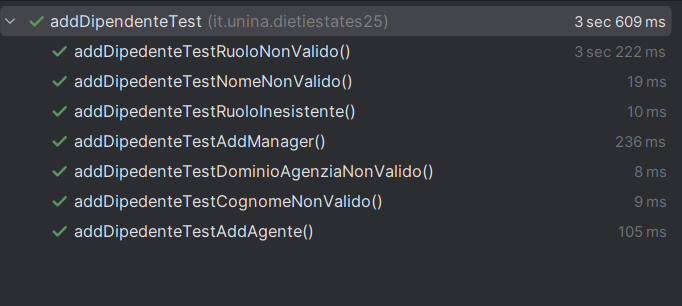
\includegraphics[width=0.7\linewidth]{Immagini/unit test/esitiTestAddDipendente.png}
	\caption[Esito test]{Screen che riporta l'esito positivo dei test}
\end{figure}


\section{utentiInteressati(CriteriDiRicercaUtenti request)}

Il metodo \colorbox{lightgray}{utentiInteressati}, appartenente alla classe \colorbox{lightgray}{RicercaAnnunciEffettuatiService}, ha la responsabilità di individuare tutti gli utenti potenzialmente interessati in base alle ricerche che essi hanno precedentemente effettuato.
Questo metodo viene invocato quando il sistema deve inviare una notifica e necessita di filtrare i destinatari realmente pertinenti. Il parametro di ingresso, \colorbox{lightgray}{CriteriDiRicercaUtenti}, contiene i campi relativi alle caratteristiche di un immobile. Se i criteri passati al metodo corrispondono a quelli di una ricerca salvata da un utente nel sistema, tale utente viene incluso nella lista dei destinatari risultanti.
\newline
Per la progettazione dei test unitari è stata adottata una \textbf{strategia di tipo black-box}, analogamente a quanto fatto per il metodo \colorbox{lightgray} {addDipendente}. Tuttavia, la motivazione alla base di questa scelta è differente: mentre nel test di \colorbox{lightgray}{addDipendente} l’obiettivo è verificare che il dipendente aggiunto possieda i valori corretti in funzione della richiesta di input, nel caso di \colorbox{lightgray}{utentiInteressati} l’attenzione è rivolta al comportamento del metodo rispetto ai criteri di ricerca forniti.
In particolare, si verifica che i valori non validi (ad esempio campi vuoti o non significativi) presenti nel parametro \colorbox{lightgray}{CriteriDiRicercaUtenti} vengano opportunamente impostati a \colorbox{lightgray}{null}, in modo da escluderli dal processo di matching con le ricerche salvate. Questo controllo è fondamentale per garantire che il sistema notifichi esclusivamente gli utenti realmente interessati.

Di seguito si riportano le tabelle che documentano tale suddivisione:

\begin{table}[H]
	\centering
	\begin{tabular}{|c|p{4cm}|p{6cm}|c|} 
		\hline
		\textbf{ID Classe} & \textbf{Descrizione} & \textbf{Valore esempio} & \textbf{Validità} \\
		\hline
		A1 & L'insieme delle stringe che corrispondo a una località italiana
		& request.areaDiInteresse==Napoli & Valido \\
		\hline
		A2 & L'insieme delle stringhe null/lunghezza zero
		& request.areaDiInteresse==null & Valido \\
		\hline
		A3 & L'insieme delle stringhe che non corrispondono a una località italiana
		& request.areaDiInteresse==città inesistente & Valido \\
		\hline
	\end{tabular}
	\caption{Parametro request.areaDiInteresse}
	\label{tab:parametriRequestAreaDiInteresse}
\end{table}

\begin{table}[H]
	\centering
	\begin{tabular}{|c|p{6cm}|p{6.2cm}|c|} 
		\hline
		\textbf{ID Classe} & \textbf{Descrizione} & \textbf{Valore esempio} & \textbf{Validità} \\
		\hline
		C1 & Un valore dell'enumerazione (AFFITTO,VENDITA)
		& request.tipoDiContrattoDiInteresse == AFFITTO; & Valido \\
		\hline
		C2 & valore null
		& request.tipoDiContrattoDiInteresse == null & Valido \\
		\hline
	\end{tabular}
	\caption{Parametro request.tipoDiContrattoDiInteresse}
	\label{tab:parametriRequestTipoDiContrattoDiInteresse}
\end{table}

\begin{table}[H]
	\centering
	\begin{tabular}{|c|p{6cm}|p{6.2cm}|c|} 
		\hline
		\textbf{ID Classe} & \textbf{Descrizione} & \textbf{Valore esempio} & \textbf{Validità} \\
		\hline
		I1 & Un valore dell'enumerazione
		& request.tipoDiImmobileDiInteresse == APPARTAMENTO; & Valido \\
		\hline
		I2 & valore null
		& request.tipoDiContrattoDiInteresse == null & Valido \\
		\hline
	\end{tabular}
	\caption{Parametro request.tipoDiImmobileDiInteresse}
	\label{tab:parametriRequestTipoDiImmobileDiInteresse}
\end{table}

\begin{table}[H]
	\centering
	\begin{tabular}{|c|p{4cm}|p{5.5cm}|c|} 
		\hline
		\textbf{ID Classe} & \textbf{Descrizione} & \textbf{Valore esempio} & \textbf{Validità} \\
		\hline
		BMI1 & Qualsiasi numero positivo
		& request.budgetMin==100 & Valido \\
		\hline
		BMI2 & qualsiasi numero negativo
		& request.budgetMin==-100 & Valido \\
		\hline
		BMI3 & valore null
		& request.budgetMin==null & Valido \\
		\hline
	\end{tabular}
	\caption{Parametro request.budgetMin}
	\label{tab:parametriRequestBudgetMin}
\end{table}

\begin{table}[H]
	\centering
	\begin{tabular}{|c|p{4cm}|p{5.5cm}|c|} 
		\hline
		\textbf{ID Classe} & \textbf{Descrizione} & \textbf{Valore esempio} & \textbf{Validità} \\
		\hline
		BMA1 & Qualsiasi numero positivo
		& request.budgetMan==600 & Valido \\
		\hline
		BMA2 & qualsiasi numero negativo
		& request.budgetMax==-600 & Valido \\
		\hline
		BMA3 & valore null
		& request.budgetMin==null & Valido \\
		\hline
	\end{tabular}
	\caption{Parametro request.budgetMax}
	\label{tab:parametriRequestBudgetMax}
\end{table}

\begin{table}[H]
	\centering
	\begin{tabular}{|c|p{4cm}|p{5.5cm}|c|} 
		\hline
		\textbf{ID Classe} & \textbf{Descrizione} & \textbf{Valore esempio} & \textbf{Validità} \\
		\hline
		IG1 & Qualsiasi intero positivo & request.intervalloGiorni==10 & Valida \\
		\hline
		II2 & intero negativo & request.intervalloGiorni==-1 & Valido \\
		\hline
		II3 & Valore null & request.intervalloGiorni==null & Valido \\
		\hline
	\end{tabular}
	\caption{Parametro request.intervalloGiorniStoricoRicerche}
	\label{tab:parametriRequestIntervalloGiorniStoricoRicerche}
\end{table}

\vspace{1cm}

% Definizione dei colori
\definecolor{bgcolor}{RGB}{245,245,245}    % Sfondo chiaro
\definecolor{keywordcolor}{RGB}{0,0,180}  % Blu per le parole chiave
\definecolor{commentcolor}{RGB}{0,128,0}  % Verde per i commenti
\definecolor{stringcolor}{RGB}{163,21,21} % Rosso per le stringhe


% Configurazione listings
\lstset{
	language=Java,                % Linguaggio di esempio
	backgroundcolor=\color{bgcolor}, % Colore di sfondo
	basicstyle=\ttfamily\small,     % Font e dimensione
	keywordstyle=\color{keywordcolor}\bfseries,
	commentstyle=\color{commentcolor}\itshape,
	stringstyle=\color{stringcolor},
	numbers=left,                   % Numeri a sinistra
	numberstyle=\tiny\color{gray},  % Stile dei numeri
	stepnumber=1,                   % Numeri in ogni riga
	numbersep=5pt,                  % Distanza dai numeri
	frame=single,                   % Cornice intorno al codice
	rulecolor=\color{gray},         % Colore della cornice
	tabsize=4,                       % Tab = 4 spazi
	showstringspaces=false,
	breaklines=true,                  % A capo automatico se troppo lungo
	literate=
		{à}{{\`a}}1
		{è}{{\`e}}1
		{é}{{\'e}}1
		{ì}{{\`i}}1
		{ò}{{\`o}}1
		{ù}{{\`u}}1
}

Prima di ogni test vengono eseguiti i settaggi di deafult della request in modo che venga modificato solo il campo di interesse i ogni test.
Mentre dopo eseguito ogni test viene verificato che alla repository, che interroga il db ed esegue il processo di corrispondenza, vengono passati i parametri che sono impostati nella request. Di seguito mostriamo il codice di tale settaggio.

\begin{lstlisting}
@BeforeEach 
void setup() {
	ricercaAnnunciEffettuataService = new RicercaAnnunciEffettuataService(mockRicercaAnnunciEffettuataRepository,MockUserRepository,new HashSet<String>());
	request = CriteriDiRicercaUtenti.builder()
	.intervalloGiorniStoricoRicerca(10)
	.tipoDiContrattoDiInteresse(TipoContratto.AFFITTO)
	.tipologiaDiImmobileDiInteresse(TipologiaImmobile.APPARTAMENTO)
	.budgetMin(BigDecimal.valueOf(100))
	.budgetMax(BigDecimal.valueOf(600))
	.areaDiInteresse("Napoli")
	.build();
}


@AfterEach 
void verifyRepositorySave() {
	verify(mockRicercaAnnunciEffettuataRepository).trovaUtentiPerCriteri(
	eq(request.getBudgetMin()),
	eq(request.getBudgetMax()),
	eq(request.getAreaDiInteresse()),
	eq(request.getTipoDiContrattoDiInteresse()),
	eq(request.getTipologiaDiImmobileDiInteresse()),
	any(LocalDateTime.class)  // qualsiasi valore va bene
	);
	
	
}
\end{lstlisting}

La suddivisione in classi di equivalenza dei parametri di questo metodo non presenta classi non valide, poiché, come spiegato, i campi con valori non validi vengono impostati a un valore specifico, come ad esempio \colorbox{lightgray}{null}.
La strategia utilizzata per la combinazione dei test consiste nel verificare tutte le classi valide con parametri validi e, successivamente, nell’eseguire un test per ciascun caso in cui un solo campo assume un valore non valido mentre tutti gli altri rimangono validi.


\begin{lstlisting}
	 /**
	* test con area di interesse Italia non deve modificare nulla tranne l'area di interesse che deve settarla a null
	*/
	@Test
	void areaDiInteresseItaliaShouldSetNullAreaDiInteresse() {
		request.setAreaDiInteresse("Italia");
		ricercaAnnunciEffettuataService.utentiInteressati(request);
		assertTrue(request.getAreaDiInteresse()==null);
	}
\end{lstlisting}

\begin{lstlisting}
	/**
	* test che controlla che se il budget max è minore del budget min, li scambia
	*/
	@Test
	void budgetMaxLessThanBudgetMinShouldSwapThem() {
		request.setBudgetMin(BigDecimal.valueOf(600));
		request.setBudgetMax(BigDecimal.valueOf(100));
		ricercaAnnunciEffettuataService.utentiInteressati(request);
		assertTrue(request.getBudgetMin().equals(BigDecimal.valueOf(100)));
		assertTrue(request.getBudgetMax().equals(BigDecimal.valueOf(600)));
	}
\end{lstlisting}

\begin{lstlisting}
	/**
	* Test che controlla che se la città non esiste, imposta a null il campo area di interesse della request
	*/
	@Test
	void invalidCityShouldSetNullAreaDiInteresse() {
		request.setAreaDiInteresse("Città Inesistente");
		ricercaAnnunciEffettuataService.utentiInteressati(request);
		assertTrue(request.getAreaDiInteresse()==null);
	}
\end{lstlisting}

\begin{lstlisting}
	/**
	* test che controlla che se budget min è negativo, lo imposta a null
	*/
	@Test
	void negativeBudgetMinShouldSetNullBudgetMin() {
		request.setBudgetMin(BigDecimal.valueOf(-100));
		ricercaAnnunciEffettuataService.utentiInteressati(request);
		
		assertTrue(request.getBudgetMin()==null);
	}
\end{lstlisting}

\begin{lstlisting}
	/**
	* test che controlla che se budget max è negativo, lo imposta a null
	*/
	@Test
	void negativeBudgetMaxShouldSetNullBudgetMax() {
		request.setBudgetMax(BigDecimal.valueOf(-100));
		ricercaAnnunciEffettuataService.utentiInteressati(request);
		assertTrue(request.getBudgetMax()==null);
	}
\end{lstlisting}

\begin{lstlisting}
	/**
	* test che controlla se l' intervallo di giorni è negativo, lo imposta setta a 7
	*/
	@Test
	void deltaDaysLessThanZeroShouldSet7() {
		request.setIntervalloGiorniStoricoRicerca(0);
		ricercaAnnunciEffettuataService.utentiInteressati(request);
		assertTrue(request.getIntervalloGiorniStoricoRicerca()==7);
		
	}
\end{lstlisting}


\begin{figure}[H]
	\centering
	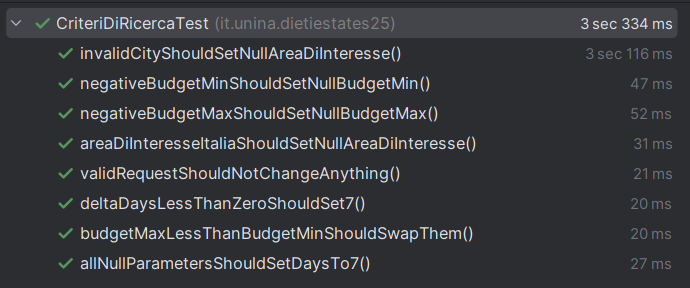
\includegraphics[width=0.7\linewidth]{Immagini/unit test/esitiTestUtentiInteressati.png}
	\caption[Esito test 2]{Screen che riporta l'esito positivo dei test}
\end{figure}


\subsection{aggiungiContatto(ContattoRequest request)}

Il metodo  \colorbox{lightgray}{aggiungiContatto()}, appartenente alla classe DatiImpiegatoService, è responsabile dell’aggiunta di un contatto di riferimento per un agente immobiliare.
Per la verifica del suo corretto funzionamento è stata adottata una \textbf{strategia di testing white-box}, poiché il metodo presenta diversi flussi di controllo interni. Questa scelta consente di verificare che, a fronte di specifici input, il metodo segua il percorso logico previsto.
\\
In particolare, il metodo deve distinguere tra due casi:
\begin{enumerate}
	\item \textbf{Il contatto esiste già}: in questo scenario, il metodo aggiorna il valore del contatto esistente.
	\item \textbf{Il contatto non esiste}: in tal caso, viene aggiunto un nuovo elemento alla lista dei contatti.
\end{enumerate}
Di seguito è riportato il \textbf{grafo del flusso di controllo (GFC)}, utilizzato per rappresentare visivamente le diverse diramazioni logiche del metodo.

\begin{figure}[H]
	\centering
	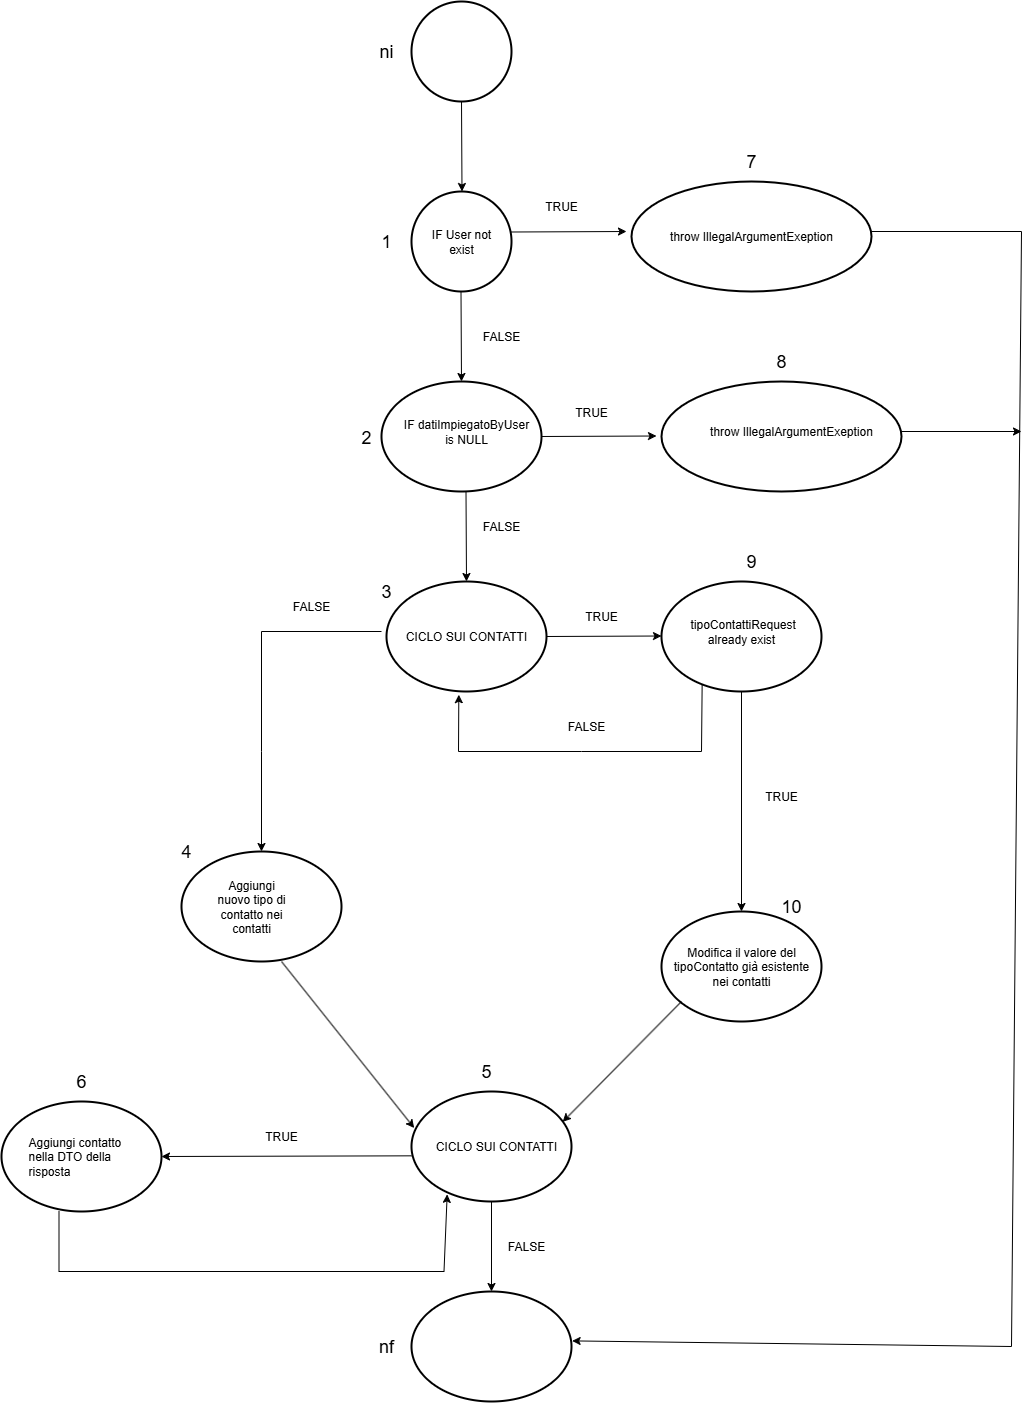
\includegraphics[width=0.7\linewidth]{Immagini/unit test/GrafoAggiungiUnContatto.png}
	\caption[GFC aggiungiContatto]{GFC del metodo aggiungiContatto(ContattoRequest request)}
\end{figure}

% Configurazione listings
\lstset{
	language=Java,                % Linguaggio di esempio
	backgroundcolor=\color{bgcolor}, % Colore di sfondo
	basicstyle=\ttfamily\small,     % Font e dimensione
	keywordstyle=\color{keywordcolor}\bfseries,
	commentstyle=\color{commentcolor}\itshape,
	stringstyle=\color{stringcolor},
	numbers=left,                   % Numeri a sinistra
	numberstyle=\tiny\color{gray},  % Stile dei numeri
	stepnumber=1,                   % Numeri in ogni riga
	numbersep=5pt,                  % Distanza dai numeri
	frame=single,                   % Cornice intorno al codice
	rulecolor=\color{gray},         % Colore della cornice
	tabsize=4,                       % Tab = 4 spazi
	showstringspaces=false,
	breaklines=true,                  % A capo automatico se troppo lungo
	literate=
	{à}{{\`a}}1
	{è}{{\`e}}1
	{é}{{\'e}}1
	{ì}{{\`i}}1
	{ò}{{\`o}}1
	{ù}{{\`u}}1
}


I test eseguiti hanno lo scopo di testare tutti i cammini possibili del grafo.

\begin{lstlisting}
	/**
	* Test verifica l'eccezione in caso di UserCurrent non trovato.
	* Copertura 1-7
	*/
	@Test
	void aggiungiContatto_ShouldThrowUnauthorizedException_
		WhenUserContextNotFound(){
		
			mocked.when(UserContex::getUserCurrent).thenReturn(null);
			
			assertThrows(it.unina.dietiestates25.exception.UnauthorizedException.class, () ->
			datiImpiegatoService.aggiungiContatto(request));
	}
\end{lstlisting}

\begin{lstlisting}
		/**
		* verifica che venga lanciata una ResourceNotFoundException quando l'utente non viene trovato nel database.
		* Copertura cammino 1-2-8
		*/
		@Test
		void aggiungiContatto_ShouldThrowResourceNotFoundException_
			WhenUserNotFoundInDB(){
			
				User mockUser = new User();
				
				mocked.when(UserContex::getUserCurrent).thenReturn(mockUser);
				when(datiImpiegatoRepository.findDatiImpiegatoByUser(mockUser)).thenReturn(Optional.empty());
				
				assertThrows(it.unina.dietiestates25.exception.ResourceNotFoundException.class, () ->
				datiImpiegatoService.aggiungiContatto(request));
			
		}
\end{lstlisting}

\begin{lstlisting}
	 /**
	* Verifica che aggiunge un nuovo contatto tra i contatti già esistenti dell'agente
	* Copertura cammino 1-2-3-4-5-6-5
	*/
	@Test
	void aggiungiContatto_
	ShouldAddNewContactWithoutExistingContacts(){
		
			request.setTipo("Cellulare");
			request.setValore("338469123");
			
			List<ContattoResponse> response = datiImpiegatoService.aggiungiContatto(request);
			
			//Controlli sul nuovo stato dei contatti esistenti dell'agente
			assertTrue(contattiEsistenti.size() == 1);
			assertTrue(contattiEsistenti.get(0).getTipo().equals("Cellulare"));
			assertTrue(contattiEsistenti.get(0).getValore().equals("338469123"));
			
			//Controlli sulla DTO in risposta
			assertTrue(response.size() == 1);
			
			assertTrue(response.get(0).getTipo().equals("Cellulare"));
			assertTrue(response.get(0).getValore().equals("338469123"));
	}
\end{lstlisting}

\begin{lstlisting}
	/**
	* Verica che aggiunge un nuovo contatto (come sopra ma con almeno un iterazione tra i contati esistenti)
	*Copertura cammino 1-2-3-9-3-4-5-6-5-6-5
	*/
	@Test
	void aggiungiContatto_
	ShouldAddNewConcatWithExistingContacts(){
		
			Contatto contatto = Contatto.builder()
			.tipo("Cellulare")
			.valore("3338469123")
			.build();
			
			contattiEsistenti.add(contatto);
			
			request.setTipo("Email");
			request.setValore("roby@gmail.com");
			
			List<ContattoResponse> response = datiImpiegatoService.aggiungiContatto(request);
			
			//Controlli sul nuovo stato dei contatti esistenti dell'agente
			assertTrue(contattiEsistenti.size() == 2);
			
			assertTrue(contattiEsistenti.get(0).getTipo().equals("Cellulare"));
			assertTrue(contattiEsistenti.get(0).getValore().equals("3338469123"));
			
			assertTrue(contattiEsistenti.get(1).getTipo().equals("Email"));
			assertTrue(contattiEsistenti.get(1).getValore().equals("roby@gmail.com"));
			
			//Controlli sulla DTO in risposta
			assertTrue(response.size() == 2);
			
			assertTrue(response.get(0).getTipo().equals("Cellulare"));
			assertTrue(response.get(0).getValore().equals("3338469123"));
			
			assertTrue(response.get(1).getTipo().equals("Email"));
			assertTrue(response.get(1).getValore().equals("roby@gmail.com"));
	}
\end{lstlisting}

\begin{lstlisting}
	/**
	* verifica che si accorge che il contatto è un tipo già esistente e quindi deve modificarne il valore non aggiungere uno nuovo.
	* Copertura cammino 1-2-3-9-3-9-10-5-6-5-6-5
	*/
	@Test
	void aggiungiContatto_ShouldModifyExistingContact(){
		
		Contatto contatto1 = Contatto.builder()
		.tipo("Cellulare")
		.valore("3338469123")
		.build();
		
		Contatto contatto2 = Contatto.builder()
		.valore("roby@gmail.com")
		.tipo("Email")
		.build();
		
		contattiEsistenti.add(contatto1);
		contattiEsistenti.add(contatto2);
		
		request.setTipo("Email");
		request.setValore("raimondo@gmail.com");
		
		List<ContattoResponse> response = datiImpiegatoService.aggiungiContatto(request);
		
		//Controlli sul nuovo stato dei contatti esistenti dell'agente
		assertTrue(contattiEsistenti.size() == 2);
		
		assertTrue(contattiEsistenti.get(0).getTipo().equals("Cellulare"));
		assertTrue(contattiEsistenti.get(0).getValore().equals("3338469123"));
		
		assertTrue(contattiEsistenti.get(1).getTipo().equals("Email"));
		assertTrue(contattiEsistenti.get(1).getValore().equals("raimondo@gmail.com"));
		
		//Controlli sulla DTO in risposta
		assertTrue(response.size() == 2);
		
		assertTrue(response.get(0).getTipo().equals("Cellulare"));
		assertTrue(response.get(0).getValore().equals("3338469123"));
		
		assertTrue(response.get(1).getTipo().equals("Email"));
		assertTrue(response.get(1).getValore().equals("raimondo@gmail.com"));
		
	}
\end{lstlisting}

\begin{lstlisting}
	  /**
	* verifica che si accorge di moficare il valore di un contatto invece di aggiungerlo uno nuovo. (Stessa verifica di sopra ma senza iterazione nel ciclo)
	* Copertura cammino 1-2-3-9-10-5-6-5
	*/
	@Test
	void aggiungiContatto_
	ShouldModifyExistingContactWithoutIteration(){
		
			Contatto contatto = Contatto.builder()
			.tipo("Cellulare")
			.valore("3338469123")
			.build();
			
			contattiEsistenti.add(contatto);
			
			request.setTipo("Cellulare");
			request.setValore("31520289137");
			
			List<ContattoResponse> response = datiImpiegatoService.aggiungiContatto(request);
			
			//Controlli sul nuovo stato dei contatti esistenti dell'agente
			assertTrue(contattiEsistenti.size() == 1);
			
			assertTrue(contattiEsistenti.get(0).getTipo().equals("Cellulare"));
			assertTrue(contattiEsistenti.get(0).getValore().equals("31520289137"));
			
			//Controlli sulla DTO in risposta
			assertTrue(response.size() == 1);
			
			assertTrue(response.get(0).getTipo().equals("Cellulare"));
			assertTrue(response.get(0).getValore().equals("31520289137"));
		
	}
\end{lstlisting}

\begin{figure}[H]
	\centering
	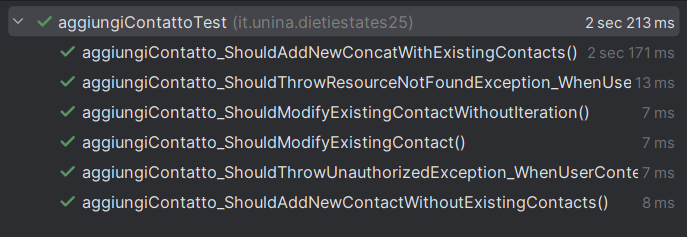
\includegraphics[width=0.7\linewidth]{Immagini/unit test/esitiTestaddContatto.png}
	\caption[Esito test 3]{Screen che riporta l'esito positivo dei test}
\end{figure}


\subsection{changePassword(String oldPassword, String newPassword, String confirmPassword)}

Il metodo \colorbox{lightgray}{changePassword}, appartenente alla classe \colorbox{lightgray}{AuthService}, è responsabile della modifica della password di un utente. Per la sua particolare struttura, si è scelto di adottare una \textbf{strategia di testing white-box}, poiché il metodo è costituito principalmente da \textbf{controlli logici} e di contesto, come la verifica della correttezza della vecchia password e la conformità della nuova password al pattern richiesto.
\\
Di seguito è riportato il \textbf{Grafo del Flusso di Controllo del metodo}, seguito dai \textbf{test case} sviluppati per garantire la copertura di \textbf{tutti i cammini possibili} all’interno del grafo.

\begin{figure}[H]
	\centering
	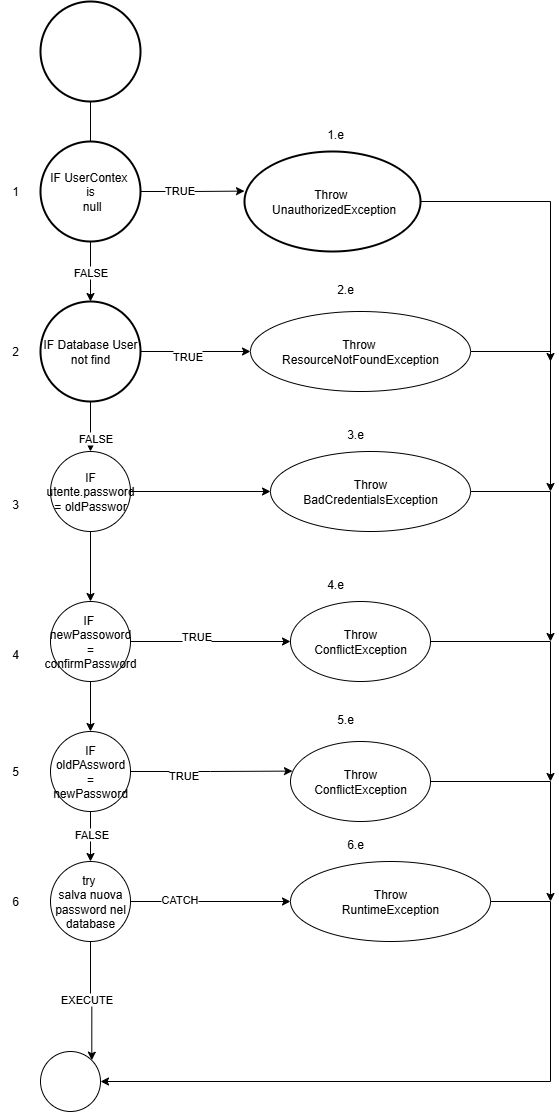
\includegraphics[width=0.7\linewidth]{Immagini/unit test/grafoCambiaPassword.png}
	\caption[GFC changePassword]{GFC del metodo changePassword(String oldPassword, String newPassword, String confirmPassword)}
\end{figure}

% Configurazione listings
\lstset{
	language=Java,                % Linguaggio di esempio
	backgroundcolor=\color{bgcolor}, % Colore di sfondo
	basicstyle=\ttfamily\small,     % Font e dimensione
	keywordstyle=\color{keywordcolor}\bfseries,
	commentstyle=\color{commentcolor}\itshape,
	stringstyle=\color{stringcolor},
	numbers=left,                   % Numeri a sinistra
	numberstyle=\tiny\color{gray},  % Stile dei numeri
	stepnumber=1,                   % Numeri in ogni riga
	numbersep=5pt,                  % Distanza dai numeri
	frame=single,                   % Cornice intorno al codice
	rulecolor=\color{gray},         % Colore della cornice
	tabsize=4,                       % Tab = 4 spazi
	showstringspaces=false,
	breaklines=true,                  % A capo automatico se troppo lungo
	literate=
	{à}{{\`a}}1
	{è}{{\`e}}1
	{é}{{\'e}}1
	{ì}{{\`i}}1
	{ò}{{\`o}}1
	{ù}{{\`u}}1
}


\begin{lstlisting}
	 /**
	*  Questo test copre i nodi da 1 al 6 percorrendo solo il cammino senza errori.
	*/
	@Test
	void changePassword_ShouldSave_WhenValid() {
		User mockUser = new User();
		mockUser.setId(1);
		
		mockUser.setPassword(passwordEncoder.encode("oldPass"));
		
		
		mocked.when(UserContex::getUserCurrent).thenReturn(mockUser);
		
		when(userRepository.findById(1)).thenReturn(Optional.of(mockUser));
		
		String result = authService.changePassword("oldPass", "newPass", "newPass");
		
		verify(userRepository).save(mockUser);
		assertEquals(Msg.PASSWORD_CHANGED, result);
		//assert true when password encorder match new password with mockUser password
		assertTrue(passwordEncoder.matches("newPass", mockUser.getPassword()));
		
	}
\end{lstlisting}

\begin{lstlisting}
	/**
	* Questo test copre il nodo 1 e 1.e
	* * verifica che venga lanciata una UnauthorizedException quando l'utente non viene trovato nel userContex.
	*/
	@Test
	void changePassword_
	ShouldThrowUnauthorizedException_WhenUserContextNotFound() {
		
		mocked.when(UserContex::getUserCurrent).thenReturn(null);
		Exception ex = assertThrows(it.unina.dietiestates25.exception.UnauthorizedException.class, () ->authService.changePassword("oldPass", "newPass", "newPass") );
	}
\end{lstlisting}
	
\begin{lstlisting}
	/**
	* Questo test copre i nodi 1, 2, 2.e
	* * verifica che venga lanciata una ResourceNotFoundException quando l'utente non viene trovato nel database.
	*/
	@Test
	void changePassword_
	ShouldThrowResourceNotFoundException_WhenUserNotFoundInDB() {
		
		User mockUser = new User();
		mockUser.setId(1);
		
		
		mocked.when(UserContex::getUserCurrent).thenReturn(mockUser);
		
		when(userRepository.findById(1)).thenReturn(Optional.empty());
		
		assertThrows(it.unina.dietiestates25.exception.ResourceNotFoundException.class, () ->authService.changePassword("oldPass", "newPass", "newPass") );
		
	}
\end{lstlisting}
	
\begin{lstlisting}
	/**
	* Questo test copre i nodi 1, 2, 3, 3.e
	* * verifica che venga lanciata una BadCredentialsException quando la vecchia password non corrisponde alla password corrente del user.
	*/
	@Test
	void changePassword_
	ShouldThrowBadCredentialsException_WhenOldPasswordNotMatch() {
		User mockUser = new User();
		mockUser.setId(1);
		mockUser.setPassword(passwordEncoder.encode("oldPass"));
		
		mocked.when(UserContex::getUserCurrent).thenReturn(mockUser);
		
		when(userRepository.findById(1)).thenReturn(Optional.of(mockUser));
		
		assertThrows(BadCredentialsException.class, () ->authService.changePassword("wrongOldPass", "newPass", "newPass") );
	}
\end{lstlisting}

\begin{lstlisting}
	/**
	* Questo test copre i nodi 1, 2, 3, 4, 4.e
	* * verifica che venga lanciata una ConflictException quando la nuova password e la password di conferma non corrispondono.
	*/
	@Test
	void changePassword_ShouldThrowConflictException
	_WhenNewPasswordNotMatchConfirmPassword() {
		
		User mockUser = new User();
		mockUser.setId(1);
		mockUser.setPassword(passwordEncoder.encode("oldPass"));
		
		mocked.when(UserContex::getUserCurrent).thenReturn(mockUser);
		
		when(userRepository.findById(1)).thenReturn(Optional.of(mockUser));
		
		assertThrows(it.unina.dietiestates25.exception.ConflictException.class, () ->authService.changePassword("oldPass", "newPass", "differentNewPass") );
	}
\end{lstlisting}

\begin{lstlisting}
	 /**
	* Questo test copre i nodi 1, 2, 3, 4, 5, 5.e
	* * verifica che venga lanciata una ConflictException quando la nuova password è uguale alla password attuale.
	*/
	@Test
	void changePassword_ShouldThrowConflictException
	_WhenNewPasswordIsSameAsOldPassword() {
		User mockUser = new User();
		mockUser.setId(1);
		mockUser.setPassword(passwordEncoder.encode("oldPass"));
		
		mocked.when(UserContex::getUserCurrent).thenReturn(mockUser);
		
		when(userRepository.findById(1)).thenReturn(Optional.of(mockUser));
		
		assertThrows(it.unina.dietiestates25.exception.ConflictException.class, () ->authService.changePassword("oldPass", "oldPass", "oldPass") );
	}
\end{lstlisting}

\begin{lstlisting}
	/**
	* Questo test copre i nodi 1, 2, 3, 4, 5, 6, 6.e
	* * verifica che venga lanciata una RuntimeException quando si verifica un errore durante il salvataggio della nuova password.
	*/
	@Test
	void changePassword_ShouldThrowRuntimeException_WhenErrorOnSave() {
		User mockUser = new User();
		
		mockUser.setId(1);
		mockUser.setPassword(passwordEncoder.encode("oldPass"));
		
		
		mocked.when(UserContex::getUserCurrent).thenReturn(mockUser);
		
		when(userRepository.findById(1)).thenReturn(Optional.of(mockUser));
		//simula un errore durante il salvataggio
		when(userRepository.save(mockUser)).thenThrow(new RuntimeException());
		
		assertThrows(RuntimeException.class, () ->authService.changePassword("oldPass", "newPass", "newPass") );
	}
\end{lstlisting}

\begin{figure}[H]
	\centering
	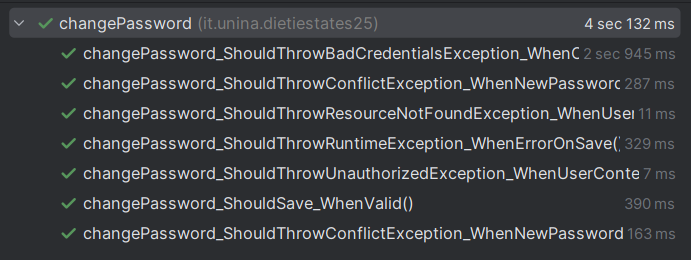
\includegraphics[width=0.7\linewidth]{Immagini/unit test/esitiTestChangePassword.png}
	\caption[Esito test 4]{Screen che riporta l'esito positivo dei test}
\end{figure}

La \textbf{valutazione dell'usabilità} rappresenta una fase essenziale nel processo di sviluppo di un’interfaccia utente, consentendo di valutare l'efficacia, l’efficienza e la soddisfazione dell’utente nell’interazione con il sistema. In particolare, l'uso di mockup interattivi offre la possibilità di raccogliere feedback sulle scelte di design prima ancora della fase di sviluppo, riducendo i costi di eventuali revisioni e migliorando la qualità dell’esperienza utente.
\newline
L'obiettivo principale di questa sezione è identificare eventuali problemi di navigazione, ambiguità nelle interazioni o difficoltà nella comprensione delle funzionalità, al fine di ottimizzare l'interfaccia prima del rilascio definitivo.

\section{Expert Reviews / Inspections}

Per valutare la qualità complessiva dell’esperienza utente e la coerenza progettuale del sistema, è stata pianificata una revisione sistematica dell’interfaccia basata su una \textbf{valutazione euristica} secondo i principi di Nielsen \cite{nielsen1995}.  
L’attività ha avuto l’obiettivo di identificare punti di forza, criticità e incoerenze nel design, analizzando in due fasi distinte il \textit{prototipo realizzato in Figma} e successivamente la \textit{versione web implementata}.  

La revisione del prototipo Figma ha rappresentato un passaggio fondamentale prima dello sviluppo effettivo: ha consentito di riflettere in modo critico sulle scelte di interfaccia, di validare le principali logiche di navigazione e di anticipare eventuali problemi di usabilità.  
A differenza della versione web, il prototipo non consente un’interazione reale, ma offre comunque una base solida per verificare la chiarezza dei flussi e la coerenza visiva complessiva.

\subsection*{Obiettivi della Review}

Gli obiettivi principali dell’attività di \textit{Expert Review} sono stati:
\begin{itemize}
    \item Valutare la \textbf{usabilità} dei flussi principali del sistema, verificando la chiarezza dei percorsi e delle azioni disponibili.
    \item Analizzare la \textbf{coerenza visiva} rispetto alle linee guida di design definite nel brand e nel prototipo.
    \item Individuare problemi di \textbf{chiarezza, navigabilità e feedback} che possano compromettere l’esperienza d’uso.
    \item Identificare eventuali mancanze o ridondanze, con l’obiettivo di \textbf{migliorare la struttura informativa e la consistenza visiva}.
    \item Definire raccomandazioni per le fasi successive di sviluppo, in vista della revisione della \textbf{versione web funzionante}.
\end{itemize}

\subsection*{Motivazione della Checklist Scelta}

Per garantire una valutazione sistematica, replicabile e comparabile tra diverse aree dell’interfaccia, è stata utilizzata una \textbf{checklist di usabilità} costruita sui dieci principi di Nielsen.  
Questo approccio è stato scelto perché:
\begin{itemize}
    \item consente una \textbf{autovalutazione strutturata} anche in assenza di utenti reali o revisori esterni;
    \item può essere applicato sia a \textbf{prototipi statici} (come quelli sviluppati in Figma) sia a \textbf{interfacce interattive} e funzionanti;
    \item copre in modo ampio le dimensioni fondamentali dell’usabilità: visibilità dello stato del sistema, coerenza, prevenzione degli errori, efficienza, chiarezza e supporto all’utente.
\end{itemize}

\subsection*{Struttura della Checklist Euristica}

La checklist adottata si basa sui dieci principi classici di Nielsen, riformulati in forma di domande operative per adattarli al contesto del progetto.  
Ogni criterio è stato utilizzato come base per analizzare il prototipo Figma e successivamente la versione web.

\begin{table}[H]
\centering
\begin{tabular}{p{0.7cm} p{4cm} p{8cm}}
\hline
\textbf{\#} & \textbf{Criterio} & \textbf{Domanda di verifica} \\
\hline
1 & Visibilità dello stato del sistema & L’utente riceve sempre un feedback visivo o testuale dopo un’azione (salvataggio, invio, errore)? \\
2 & Corrispondenza tra sistema e mondo reale & Terminologia, icone e messaggi sono coerenti con il linguaggio del dominio immobiliare? \\
3 & Controllo e libertà dell’utente & È possibile annullare o correggere facilmente un’azione? \\
4 & Coerenza e standard & Colori, stili e componenti rispettano il design definito nel brand e nel prototipo? \\
5 & Prevenzione e gestione degli errori & I form prevengono gli errori tramite validazioni e messaggi chiari? \\
6 & Efficienza e flessibilità d’uso & Le operazioni più frequenti possono essere eseguite rapidamente, anche da dispositivi mobili? \\
7 & Chiarezza del contenuto & Testi e etichette sono comprensibili e privi di ambiguità? \\
8 & Supporto al riconoscimento & Le opzioni principali sono visibili e non richiedono memoria a breve termine all’utente? \\
9 & Feedback e conferme & Sono presenti messaggi di conferma dopo azioni critiche (pubblicazione, eliminazione, invio)? \\
10 & Aiuto e documentazione & È disponibile un supporto o una guida per l’utente in caso di difficoltà? \\
\hline
\end{tabular}
\caption{Checklist di valutazione euristica basata sui principi di Nielsen.}
\end{table}

\bigskip

La sezione seguente presenta nel dettaglio l’applicazione di questa checklist al \textbf{prototipo Figma}, con un’analisi critica dei dieci criteri e una successiva autovalutazione sintetica dei risultati ottenuti.

\subsection{Expert Review sul Prototipo Figma}

L’attività di revisione euristica è stata condotta sul prototipo sviluppato in \textit{Figma} prima della realizzazione della versione web.  
L’obiettivo è stato valutare il livello di usabilità e coerenza delle principali interfacce progettate, verificando la presenza di feedback, la chiarezza dei flussi e la consistenza grafica secondo i dieci principi di Nielsen.  

\subsubsection*{1. Visibilità dello stato del sistema}  
Nel prototipo sono stati previsti diversi meccanismi di feedback.  
Nei flussi \textit{Fai controproposta} e \textit{Registra dipendente} sono stati inseriti \textbf{indicatori di caricamento} per mostrare lo stato del sistema durante le operazioni.  
In tutti i form è presente un \textbf{sistema di validazione immediata}: i campi non validi vengono evidenziati in rosso e, nel caso della \textit{creazione di un annuncio}, il processo è suddiviso in step.  
Quando uno step contiene errori, il suo indicatore cambia colore e un box iniziale riepiloga i campi non validi.  
Tutti i flussi analizzati includono un \textbf{doppio messaggio di conferma} prima dell’esecuzione definitiva, ad eccezione della creazione di un annuncio.  
Nel complesso, il prototipo offre una buona visibilità dello stato del sistema, con l’unica criticità relativa all’assenza di conferma dopo la pubblicazione.

\subsubsection*{2. Corrispondenza tra sistema e mondo reale}  
Il linguaggio utilizzato è \textbf{semplice e diretto}, adatto agli utenti finali.  
Le sezioni con terminologia più specifica (legate alle agenzie immobiliari) risultano coerenti con il dominio e adatte a un pubblico professionale.  
Sono state impiegate \textbf{icone standard e universalmente riconoscibili}, affiancate da \textbf{tooltip descrittivi} che ne chiariscono il significato.  
L’unico aspetto ancora da migliorare riguarda la \textbf{scelta delle icone nello stepper} di creazione annuncio, dove sarebbe utile uno studio mirato per rendere più intuitivi i passaggi.

\subsubsection*{3. Controllo e libertà dell’utente}  
Il prototipo garantisce buone possibilità di annullamento e controllo.  
Tutti i popup includono una \textbf{“X” per chiudere o annullare}, e i messaggi di conferma prevedono esplicitamente un pulsante \textit{Annulla}.  
Le azioni potenzialmente distruttive, come la \textbf{disattivazione delle notifiche}, richiedono conferma; viceversa, l’attivazione non la richiede poiché non comporta rischi di perdita di dati.  
La progettazione su questo punto è stata ritenuta soddisfacente e coerente con le aspettative di usabilità.

\subsubsection*{4. Coerenza e standard}  
Il design mantiene nel complesso una \textbf{coerenza visiva} nei colori e nello stile dei pulsanti, in linea con il concept minimalista del progetto.  
Tuttavia, si è rilevata una \textbf{mancanza di uniformità nei popup}: nei diversi casi d’uso sono stati utilizzati modelli leggermente differenti, frutto di sperimentazioni grafiche ancora non consolidate.  
In fase di sviluppo sarà necessario \textbf{uniformare componenti e modali}, garantendo una coerenza piena tra tutti i flussi.

\subsubsection*{5. Prevenzione e gestione degli errori}  
La prevenzione degli errori è uno degli aspetti più curati nel prototipo.  
I form mostrano in tempo reale i campi non validi e forniscono \textbf{indicazioni visive chiare (rosso)} insieme a messaggi testuali.  
La combinazione di validazione immediata e conferme d’azione riduce significativamente il rischio di errori da parte dell’utente.  
Questo punto risulta pienamente soddisfatto.

\subsubsection*{6. Efficienza e flessibilità d’uso}  
Essendo un prototipo statico, l’efficienza d’uso è valutabile solo in parte.  
L’interfaccia è stata progettata per un utilizzo anche da \textbf{dispositivi verticali}, ma la resa migliore si ottiene in \textbf{orientamento orizzontale (landscape)}.  
Non sono state ancora considerate \textbf{scorciatoie o funzionalità avanzate} per utenti esperti (es. salvataggio bozza, importazione di dati da file), che potrebbero rappresentare un’evoluzione futura del progetto.  
Si riconosce quindi questo come un punto da sviluppare ulteriormente.

\subsubsection*{7. Chiarezza del contenuto}  
I testi sono \textbf{brevi, diretti e privi di tecnicismi}, con un linguaggio coerente e immediato.  
Quando una sola etichetta non è sufficiente, è previsto l’uso di \textbf{tooltip esplicativi}.  
Questo approccio consente una buona comprensione del flusso anche senza documentazione aggiuntiva.

\subsubsection*{8. Supporto al riconoscimento}  
Le principali funzioni sono \textbf{raggiungibili in pochi clic}.  
La \textit{header bar} consente di passare rapidamente tra ricerca, storico annunci e notifiche; inoltre, il passaggio tra l’area cliente e quella agenzia è reso accessibile dal \textit{footer}.  
Un test di eye-tracking condotto su alcune schermate del prototipo ha confermato la \textbf{corretta collocazione visiva} degli elementi più rilevanti, validando l’efficacia della struttura.

\subsubsection*{9. Feedback e conferme}  
Le operazioni critiche, come eliminazione o modifica, utilizzano lo stesso colore principale del sito, il che può generare confusione con azioni neutre.  
Si suggerisce di differenziare \textbf{visivamente le azioni distruttive} (es. usando toni di rosso o arancione) e di inserire messaggi di conferma più evidenti per i processi più delicati.  
Nonostante ciò, il comportamento rimane accettabile per utenti esperti.

\subsubsection*{10. Aiuto e documentazione}  
Non è stato previsto un sistema di aiuto, documentazione o FAQ, poiché il prototipo nasce in un contesto accademico.  
Tuttavia, in una versione completa sarebbe opportuno introdurre:  
\begin{itemize}
    \item una \textbf{sezione FAQ} o assistenza per i problemi più comuni;  
    \item \textbf{overlay o onboarding guidato} per i nuovi utenti;  
    \item pulsanti contestuali “Come funziona” nelle pagine più complesse.  
\end{itemize}

\subsubsection*{Autovalutazione e sintesi}  
La tabella seguente riassume il livello di soddisfacimento delle euristiche sul prototipo Figma (0 = non soddisfatto, 1 = parzialmente soddisfatto, 2 = soddisfatto).

\begin{table}[h!]
\centering
\begin{tabular}{p{0.4cm} p{4cm} p{1.5cm} p{7cm}}
\hline
\textbf{\#} & \textbf{Criterio} & \textbf{Valutazione} & \textbf{Motivazione sintetica} \\ \hline
1 & Visibilità stato & 2 & Feedback e validazioni chiare, manca solo conferma finale in creazione annuncio \\
2 & Corrispondenza mondo reale & 2 & Linguaggio semplice e coerente, icone chiare \\
3 & Controllo e libertà & 2 & Annulla e conferme sempre presenti \\
4 & Coerenza e standard & 1 & Popup non uniformi tra i flussi \\
5 & Prevenzione errori & 2 & Validazione in tempo reale e segnalazioni visive \\
6 & Efficienza/flessibilità & 1 & Assenza di scorciatoie e ottimizzazione solo parziale per mobile \\
7 & Chiarezza del contenuto & 2 & Testi sintetici e coerenti \\
8 & Supporto al riconoscimento & 2 & Navigazione semplice e confermata da test visivi \\
9 & Feedback/Conferme & 1 & Colori azioni critiche da differenziare \\
10 & Aiuto/Documentazione & 0 & Non prevista sezione di supporto \\ \hline
\end{tabular}
\caption{Autovalutazione euristica del prototipo Figma secondo i principi di Nielsen.}
\end{table}

\subsubsection*{Conclusioni}  
Il prototipo Figma risulta \textbf{completo, coerente e ben strutturato}, con una gestione accurata dei form, validazioni efficaci e buona leggibilità generale.  
I principali margini di miglioramento riguardano la \textbf{coerenza visiva dei popup}, la \textbf{differenziazione dei feedback critici} e l’assenza di un \textbf{sistema di aiuto} o onboarding.  
Questi aspetti costituiranno la base per le iterazioni successive e per l’ottimizzazione della versione web finale.



TODO Da fare bene la seocnda parte 

\textbf{Versione Web:} la checklist è stata applicata all’intero insieme di requisiti e funzionalità richiesti dal docente, permettendo una valutazione completa dell’interfaccia e dei flussi principali del sistema.

\subsection*{Definizione della Checklist di Usabilità}

La checklist elaborata si basa su una selezione adattata delle euristiche di Nielsen, ridotte e riformulate per meglio aderire al contesto del progetto.  
Ogni criterio è espresso come domanda di verifica utilizzata per valutare sia il prototipo sia il sito web.

\begin{table}[h!]
\centering
\begin{tabular}{p{0.8cm} p{4cm} p{7cm}}
\hline
\textbf{\#} & \textbf{Criterio} & \textbf{Domanda di verifica} \\
\hline
1 & Visibilità dello stato del sistema & L’utente riceve sempre un feedback visivo o testuale in seguito a un’azione (es. salvataggio, invio, errore)? \\
2 & Corrispondenza tra sistema e mondo reale & Terminologia, icone e messaggi sono coerenti con il linguaggio del dominio immobiliare? \\
3 & Controllo e libertà dell’utente & È possibile annullare o correggere facilmente un’azione (es. modifica o cancellazione di un annuncio)? \\
4 & Coerenza e standard & Colori, stili e pulsanti rispettano il design definito nel brand e nel prototipo Figma? \\
5 & Prevenzione e gestione degli errori & I form prevengono errori tramite validazioni e messaggi chiari? \\
6 & Efficienza e flessibilità d’uso & Le operazioni più frequenti possono essere completate rapidamente e da dispositivi mobili verticali? \\
7 & Chiarezza del contenuto & I testi e le etichette guidano l’utente nel flusso, senza ambiguità? \\
8 & Supporto al riconoscimento & Le opzioni principali sono sempre visibili senza richiedere memoria a breve termine all’utente? \\
9 & Feedback e conferme & Sono presenti messaggi di conferma dopo operazioni critiche (es. pubblicazione, eliminazione, invio)? \\
10 & Aiuto e documentazione & È disponibile una sezione informativa o un supporto base per l’utente? \\
\hline
\end{tabular}
\caption{Checklist di usabilità basata sulle euristiche di Nielsen, adattata al contesto del sito immobiliare multi-agenzia.}
\label{tab:checklist_usabilita}
\end{table}

\subsection*{Applicazione della Checklist}

La review è stata eseguita individualmente per ciascun caso d’uso su Figma e per l’intero insieme di funzionalità sulla versione web.  
I risultati sono stati successivamente confrontati per identificare le criticità più significative e le aree di miglioramento.




\section{Expert Reviews / Inspections}

Per valutare la qualità complessiva dell’esperienza utente e la coerenza progettuale del sistema, è stata pianificata una revisione sistematica dell’interfaccia basata su una \textbf{valutazione euristica} secondo i principi di Nielsen \cite{nielsen1995}.  
L’attività ha avuto l’obiettivo di identificare punti di forza, criticità e incoerenze nel design, analizzando in due fasi distinte il \textit{prototipo realizzato in Figma} e successivamente la \textit{versione web implementata}.  

La revisione del prototipo Figma ha rappresentato un passaggio fondamentale prima dello sviluppo effettivo: ha consentito di riflettere in modo critico sulle scelte di interfaccia, di validare le principali logiche di navigazione e di anticipare eventuali problemi di usabilità.  
A differenza della versione web, il prototipo non consente un’interazione reale, ma offre comunque una base solida per verificare la chiarezza dei flussi e la coerenza visiva complessiva.

\subsection*{Obiettivi della Review}

Gli obiettivi principali dell’attività di \textit{Expert Review} sono stati:
\begin{itemize}
    \item Valutare la \textbf{usabilità} dei flussi principali del sistema, verificando la chiarezza dei percorsi e delle azioni disponibili.
    \item Analizzare la \textbf{coerenza visiva} rispetto alle linee guida di design definite nel brand e nel prototipo.
    \item Individuare problemi di \textbf{chiarezza, navigabilità e feedback} che possano compromettere l’esperienza d’uso.
    \item Identificare eventuali mancanze o ridondanze, con l’obiettivo di \textbf{migliorare la struttura informativa e la consistenza visiva}.
    \item Definire raccomandazioni per le fasi successive di sviluppo, in vista della revisione della \textbf{versione web funzionante}.
\end{itemize}

\subsection*{Motivazione della Checklist Scelta}

Per garantire una valutazione sistematica, replicabile e comparabile tra diverse aree dell’interfaccia, è stata utilizzata una \textbf{checklist di usabilità} costruita sui dieci principi di Nielsen.  
Questo approccio è stato scelto perché:
\begin{itemize}
    \item consente una \textbf{autovalutazione strutturata} anche in assenza di utenti reali o revisori esterni;
    \item può essere applicato sia a \textbf{prototipi statici} (come quelli sviluppati in Figma) sia a \textbf{interfacce interattive} e funzionanti;
    \item copre in modo ampio le dimensioni fondamentali dell’usabilità: visibilità dello stato del sistema, coerenza, prevenzione degli errori, efficienza, chiarezza e supporto all’utente.
\end{itemize}

\subsection*{Struttura della Checklist Euristica}

La checklist adottata si basa sui dieci principi classici di Nielsen, riformulati in forma di domande operative per adattarli al contesto del progetto.  
Ogni criterio è stato utilizzato come base per analizzare il prototipo Figma e successivamente la versione web.

\begin{table}[H]
\centering
\begin{tabular}{p{0.7cm} p{4cm} p{8cm}}
\hline
\textbf{\#} & \textbf{Criterio} & \textbf{Domanda di verifica} \\
\hline
1 & Visibilità dello stato del sistema & L’utente riceve sempre un feedback visivo o testuale dopo un’azione (salvataggio, invio, errore)? \\
2 & Corrispondenza tra sistema e mondo reale & Terminologia, icone e messaggi sono coerenti con il linguaggio del dominio immobiliare? \\
3 & Controllo e libertà dell’utente & È possibile annullare o correggere facilmente un’azione? \\
4 & Coerenza e standard & Colori, stili e componenti rispettano il design definito nel brand e nel prototipo? \\
5 & Prevenzione e gestione degli errori & I form prevengono gli errori tramite validazioni e messaggi chiari? \\
6 & Efficienza e flessibilità d’uso & Le operazioni più frequenti possono essere eseguite rapidamente, anche da dispositivi mobili? \\
7 & Chiarezza del contenuto & Testi e etichette sono comprensibili e privi di ambiguità? \\
8 & Supporto al riconoscimento & Le opzioni principali sono visibili e non richiedono memoria a breve termine all’utente? \\
9 & Feedback e conferme & Sono presenti messaggi di conferma dopo azioni critiche (pubblicazione, eliminazione, invio)? \\
10 & Aiuto e documentazione & È disponibile un supporto o una guida per l’utente in caso di difficoltà? \\
\hline
\end{tabular}
\caption{Checklist di valutazione euristica basata sui principi di Nielsen.}
\end{table}

\bigskip

La sezione seguente presenta nel dettaglio l’applicazione di questa checklist al \textbf{prototipo Figma}, con un’analisi critica dei dieci criteri e una successiva autovalutazione sintetica dei risultati ottenuti.

\subsection{Expert Review sul Prototipo Figma}

L’attività di revisione euristica è stata condotta sul prototipo sviluppato in \textit{Figma} prima della realizzazione della versione web.  
L’obiettivo è stato valutare il livello di usabilità e coerenza delle principali interfacce progettate, verificando la presenza di feedback, la chiarezza dei flussi e la consistenza grafica secondo i dieci principi di Nielsen.  

\subsubsection*{1. Visibilità dello stato del sistema}  
Nel prototipo sono stati previsti diversi meccanismi di feedback.  
Nei flussi \textit{Fai controproposta} e \textit{Registra dipendente} sono stati inseriti \textbf{indicatori di caricamento} per mostrare lo stato del sistema durante le operazioni.  
In tutti i form è presente un \textbf{sistema di validazione immediata}: i campi non validi vengono evidenziati in rosso e, nel caso della \textit{creazione di un annuncio}, il processo è suddiviso in step.  
Quando uno step contiene errori, il suo indicatore cambia colore e un box iniziale riepiloga i campi non validi.  
Tutti i flussi analizzati includono un \textbf{doppio messaggio di conferma} prima dell’esecuzione definitiva, ad eccezione della creazione di un annuncio.  
Nel complesso, il prototipo offre una buona visibilità dello stato del sistema, con l’unica criticità relativa all’assenza di conferma dopo la pubblicazione.

\subsubsection*{2. Corrispondenza tra sistema e mondo reale}  
Il linguaggio utilizzato è \textbf{semplice e diretto}, adatto agli utenti finali.  
Le sezioni con terminologia più specifica (legate alle agenzie immobiliari) risultano coerenti con il dominio e adatte a un pubblico professionale.  
Sono state impiegate \textbf{icone standard e universalmente riconoscibili}, affiancate da \textbf{tooltip descrittivi} che ne chiariscono il significato.  
L’unico aspetto ancora da migliorare riguarda la \textbf{scelta delle icone nello stepper} di creazione annuncio, dove sarebbe utile uno studio mirato per rendere più intuitivi i passaggi.

\subsubsection*{3. Controllo e libertà dell’utente}  
Il prototipo garantisce buone possibilità di annullamento e controllo.  
Tutti i popup includono una \textbf{“X” per chiudere o annullare}, e i messaggi di conferma prevedono esplicitamente un pulsante \textit{Annulla}.  
Le azioni potenzialmente distruttive, come la \textbf{disattivazione delle notifiche}, richiedono conferma; viceversa, l’attivazione non la richiede poiché non comporta rischi di perdita di dati.  
La progettazione su questo punto è stata ritenuta soddisfacente e coerente con le aspettative di usabilità.

\subsubsection*{4. Coerenza e standard}  
Il design mantiene nel complesso una \textbf{coerenza visiva} nei colori e nello stile dei pulsanti, in linea con il concept minimalista del progetto.  
Tuttavia, si è rilevata una \textbf{mancanza di uniformità nei popup}: nei diversi casi d’uso sono stati utilizzati modelli leggermente differenti, frutto di sperimentazioni grafiche ancora non consolidate.  
In fase di sviluppo sarà necessario \textbf{uniformare componenti e modali}, garantendo una coerenza piena tra tutti i flussi.

\subsubsection*{5. Prevenzione e gestione degli errori}  
La prevenzione degli errori è uno degli aspetti più curati nel prototipo.  
I form mostrano in tempo reale i campi non validi e forniscono \textbf{indicazioni visive chiare (rosso)} insieme a messaggi testuali.  
La combinazione di validazione immediata e conferme d’azione riduce significativamente il rischio di errori da parte dell’utente.  
Questo punto risulta pienamente soddisfatto.

\subsubsection*{6. Efficienza e flessibilità d’uso}  
Essendo un prototipo statico, l’efficienza d’uso è valutabile solo in parte.  
L’interfaccia è stata progettata per un utilizzo anche da \textbf{dispositivi verticali}, ma la resa migliore si ottiene in \textbf{orientamento orizzontale (landscape)}.  
Non sono state ancora considerate \textbf{scorciatoie o funzionalità avanzate} per utenti esperti (es. salvataggio bozza, importazione di dati da file), che potrebbero rappresentare un’evoluzione futura del progetto.  
Si riconosce quindi questo come un punto da sviluppare ulteriormente.

\subsubsection*{7. Chiarezza del contenuto}  
I testi sono \textbf{brevi, diretti e privi di tecnicismi}, con un linguaggio coerente e immediato.  
Quando una sola etichetta non è sufficiente, è previsto l’uso di \textbf{tooltip esplicativi}.  
Questo approccio consente una buona comprensione del flusso anche senza documentazione aggiuntiva.

\subsubsection*{8. Supporto al riconoscimento}  
Le principali funzioni sono \textbf{raggiungibili in pochi clic}.  
La \textit{header bar} consente di passare rapidamente tra ricerca, storico annunci e notifiche; inoltre, il passaggio tra l’area cliente e quella agenzia è reso accessibile dal \textit{footer}.  
Un test di eye-tracking condotto su alcune schermate del prototipo ha confermato la \textbf{corretta collocazione visiva} degli elementi più rilevanti, validando l’efficacia della struttura.

\subsubsection*{9. Feedback e conferme}  
Le operazioni critiche, come eliminazione o modifica, utilizzano lo stesso colore principale del sito, il che può generare confusione con azioni neutre.  
Si suggerisce di differenziare \textbf{visivamente le azioni distruttive} (es. usando toni di rosso o arancione) e di inserire messaggi di conferma più evidenti per i processi più delicati.  
Nonostante ciò, il comportamento rimane accettabile per utenti esperti.

\subsubsection*{10. Aiuto e documentazione}  
Non è stato previsto un sistema di aiuto, documentazione o FAQ, poiché il prototipo nasce in un contesto accademico.  
Tuttavia, in una versione completa sarebbe opportuno introdurre:  
\begin{itemize}
    \item una \textbf{sezione FAQ} o assistenza per i problemi più comuni;  
    \item \textbf{overlay o onboarding guidato} per i nuovi utenti;  
    \item pulsanti contestuali “Come funziona” nelle pagine più complesse.  
\end{itemize}

\subsubsection*{Autovalutazione e sintesi}  
La tabella seguente riassume il livello di soddisfacimento delle euristiche sul prototipo Figma (0 = non soddisfatto, 1 = parzialmente soddisfatto, 2 = soddisfatto).

\begin{table}[h!]
\centering
\begin{tabular}{p{0.4cm} p{4cm} p{1.5cm} p{7cm}}
\hline
\textbf{\#} & \textbf{Criterio} & \textbf{Valutazione} & \textbf{Motivazione sintetica} \\ \hline
1 & Visibilità stato & 2 & Feedback e validazioni chiare, manca solo conferma finale in creazione annuncio \\
2 & Corrispondenza mondo reale & 2 & Linguaggio semplice e coerente, icone chiare \\
3 & Controllo e libertà & 2 & Annulla e conferme sempre presenti \\
4 & Coerenza e standard & 1 & Popup non uniformi tra i flussi \\
5 & Prevenzione errori & 2 & Validazione in tempo reale e segnalazioni visive \\
6 & Efficienza/flessibilità & 1 & Assenza di scorciatoie e ottimizzazione solo parziale per mobile \\
7 & Chiarezza del contenuto & 2 & Testi sintetici e coerenti \\
8 & Supporto al riconoscimento & 2 & Navigazione semplice e confermata da test visivi \\
9 & Feedback/Conferme & 1 & Colori azioni critiche da differenziare \\
10 & Aiuto/Documentazione & 0 & Non prevista sezione di supporto \\ \hline
\end{tabular}
\caption{Autovalutazione euristica del prototipo Figma secondo i principi di Nielsen.}
\end{table}

\subsubsection*{Conclusioni}  
Il prototipo Figma risulta \textbf{completo, coerente e ben strutturato}, con una gestione accurata dei form, validazioni efficaci e buona leggibilità generale.  
I principali margini di miglioramento riguardano la \textbf{coerenza visiva dei popup}, la \textbf{differenziazione dei feedback critici} e l’assenza di un \textbf{sistema di aiuto} o onboarding.  
Questi aspetti costituiranno la base per le iterazioni successive e per l’ottimizzazione della versione web finale.



TODO Da fare bene la seocnda parte 

\textbf{Versione Web:} la checklist è stata applicata all’intero insieme di requisiti e funzionalità richiesti dal docente, permettendo una valutazione completa dell’interfaccia e dei flussi principali del sistema.

\subsection*{Definizione della Checklist di Usabilità}

La checklist elaborata si basa su una selezione adattata delle euristiche di Nielsen, ridotte e riformulate per meglio aderire al contesto del progetto.  
Ogni criterio è espresso come domanda di verifica utilizzata per valutare sia il prototipo sia il sito web.

\begin{table}[h!]
\centering
\begin{tabular}{p{0.8cm} p{4cm} p{7cm}}
\hline
\textbf{\#} & \textbf{Criterio} & \textbf{Domanda di verifica} \\
\hline
1 & Visibilità dello stato del sistema & L’utente riceve sempre un feedback visivo o testuale in seguito a un’azione (es. salvataggio, invio, errore)? \\
2 & Corrispondenza tra sistema e mondo reale & Terminologia, icone e messaggi sono coerenti con il linguaggio del dominio immobiliare? \\
3 & Controllo e libertà dell’utente & È possibile annullare o correggere facilmente un’azione (es. modifica o cancellazione di un annuncio)? \\
4 & Coerenza e standard & Colori, stili e pulsanti rispettano il design definito nel brand e nel prototipo Figma? \\
5 & Prevenzione e gestione degli errori & I form prevengono errori tramite validazioni e messaggi chiari? \\
6 & Efficienza e flessibilità d’uso & Le operazioni più frequenti possono essere completate rapidamente e da dispositivi mobili verticali? \\
7 & Chiarezza del contenuto & I testi e le etichette guidano l’utente nel flusso, senza ambiguità? \\
8 & Supporto al riconoscimento & Le opzioni principali sono sempre visibili senza richiedere memoria a breve termine all’utente? \\
9 & Feedback e conferme & Sono presenti messaggi di conferma dopo operazioni critiche (es. pubblicazione, eliminazione, invio)? \\
10 & Aiuto e documentazione & È disponibile una sezione informativa o un supporto base per l’utente? \\
\hline
\end{tabular}
\caption{Checklist di usabilità basata sulle euristiche di Nielsen, adattata al contesto del sito immobiliare multi-agenzia.}
\label{tab:checklist_usabilita}
\end{table}

\subsection*{Applicazione della Checklist}

La review è stata eseguita individualmente per ciascun caso d’uso su Figma e per l’intero insieme di funzionalità sulla versione web.  
I risultati sono stati successivamente confrontati per identificare le criticità più significative e le aree di miglioramento.


